\documentclass[11pt]{article}

\usepackage[utf8]{inputenc}
\usepackage[T1]{fontenc}
\usepackage{lmodern}
\usepackage{amsmath,amssymb,amsthm}
\usepackage{geometry}
\usepackage{microtype}
\usepackage{setspace}
\usepackage{graphicx}
\usepackage[round,authoryear]{natbib}
\usepackage{hyperref}
\geometry{margin=1.15in}
\onehalfspacing

\newtheorem{proposition}{Proposition}
\theoremstyle{definition}
\newtheorem{definition}{Definition}

\newcommand{\E}{\mathbb{E}}
\newcommand{\bB}{\mathbf{B}}
\newcommand{\bM}{\mathbf{M}}
\newcommand{\bI}{\mathbf{I}}
\newcommand{\bQ}{\mathbf{Q}}

\title{Regularity Without Invariance:\\The Limits of the Interhemispheric Monsoon Dipole}
\author{Flyxion\\Independent Researcher}
\date{October 2026}

\begin{document}
\maketitle

\begin{abstract}
\noindent
The global monsoon is commonly understood through the interhemispheric redistribution of seasonal heating and tropical precipitation. Orbital precession favours alternating monsoon intensification between hemispheres, producing a persistent climatic dipole. A 450,000-year South American speleothem record presented by \citet{olson2026}, compared with Asian monsoon records, confirms this dominant opposition while identifying ten intervals of anomalous interhemispheric synchronicity. During several warm or warming intervals, both monsoons weakened for periods lasting up to several millennia, challenging the sufficiency of a displacement-only account in which a weakening northern monsoon is accompanied by southern intensification. This essay examines the physical and explanatory significance of these events. It distinguishes the conservation of atmospheric moisture and energy from the nonconservation of regional rainfall, develops a common-mode and difference-mode representation of monsoon variability, and considers whether synchronous anomalies reflect common forcing, state-dependent coupling, or nonlinear dynamical transitions. It argues that the evidence establishes the conditional character of the interhemispheric dipole without yet demonstrating a bifurcation or a distinct climatic attractor. The resulting framework clarifies how persistent climatic regularities may remain predictive within established boundary conditions while failing under their reorganization.
\end{abstract}

\section{Introduction: The Regularity and Its Exceptions}

The interhemispheric monsoon dipole refers to the tendency of Northern and Southern Hemisphere summer monsoons to vary in opposing phases, principally in response to orbital changes in seasonal solar radiation. This opposition is a persistent feature of the palaeoclimate record, but it is neither a conservation law nor an invariant relationship. Its expression depends on the oceanic, atmospheric, and cryospheric conditions under which orbital forcing operates.

For most of the past 450,000 years the Asian and South American summer monsoons have varied in approximately opposite phases. When the Asian monsoon was strong, the South American monsoon tended to be weak, and the reverse held when the orbital configuration shifted. This opposition follows the seasonal redistribution of solar radiation produced by Earth's orbital precession, and it is strongly supported by the palaeoclimate record. A speleothem sequence assembled from three caves on the eastern flank of the Peruvian Andes and compared with the well-known Asian cave records by \citet{olson2026} reproduces the opposition over several glacial cycles, and it does so with enough fidelity that the dipole can be treated as the baseline expectation against which any other behaviour must be measured. Even this baseline is not uniform. The authors report that the mirror-image relation weakens markedly during Marine Isotope Stage 11, an interval of weak precessional forcing in which the two monsoons no longer closely mirror one another.

The same record contains intervals that do not fit the baseline. Olson and colleagues identify ten episodes, defined by a synchronicity threshold, in which the Asian and South American monsoons departed from opposition and moved together. The research briefing that accompanies the article reports that during periods of rapid global warming or warmth the two systems weakened synchronously for intervals of 100 to 4,250 years, and that during especially cold glacial conditions they strengthened in unison. The exceptions are not marginal in character. A simplified interpretation of hemispheric redistribution suggests that a displacement of tropical convection toward one hemisphere should favour monsoon intensification there while suppressing rainfall in the other. This expectation is physically motivated but conditional. It does not follow from the conservation of atmospheric moisture or energy that precipitation anomalies in two selected monsoon regions must cancel. Concurrent weakening in both hemispheres therefore challenges the sufficiency of a displacement-only explanation, and not the conservation principles on which atmospheric dynamics rests, so the episodes bear on how the regularity should be understood and not merely on how well it fits.

The argument of this essay begins from a distinction that is easily lost when a pattern has held for a very long time. A regularity observed under prevailing conditions is one thing, and a relation that remains invariant when those conditions change is another. The first is an empirical description of how a system has behaved within a certain range of states. The second is a claim about the structure of the system that holds across states. Orbital forcing has organized the interhemispheric monsoon dipole for hundreds of thousands of years, but the long persistence of a pattern cannot by itself establish that the pattern is unconditional. A relation that survived because the surrounding boundary conditions happened to remain within a favourable range could be observationally indistinguishable, over the range of states actually sampled, from an invariant law.

The word invariance can be taken in several senses: constancy of a response coefficient, constancy of the sign of a relationship, constancy under changes of boundary conditions, and constancy of the physical laws themselves. Only one of these is at issue. Invariance here means the persistence of a specified relation between forcing and response across changes in climatic background state. It does not mean the invariance of the governing conservation laws, nor does it require that the response be numerically identical at every point in time.

The essay therefore proceeds by separating three questions that discussions of anomalous climatic episodes often run together. The first concerns forcing: whether some additional external influence was applied to the system during the synchronous intervals. The second concerns coupling: whether the strength or sign of the response to a given forcing changed because the state of the oceans, ice sheets, and atmosphere changed. The third concerns dynamical organization: whether the system crossed a stability threshold and settled into a qualitatively different configuration. These possibilities have different physical content, different observational signatures, and very different implications for prediction. The principal question that follows is what the temporary failure of a persistent climatic dipole reveals about the organization, stability, and predictability of coupled systems.

The treatment is organized in the following way. Sections~II and~III establish the astronomical explanation of the dipole and the evidential basis of the speleothem record, taking care to present the conventional account at full strength. Section~IV describes the ten departures and what synchronicity does and does not mean. Section~V argues that the departures violate a simplified model of the physics and not the physics itself, because redistribution of atmospheric water is not a conservation law for rainfall in two chosen regions. Section~VI introduces oceanic teleconnections and the idea of conditional coupling. Section~VII develops a mathematical interpretation in terms of common and difference modes; this interpretation is the author's own, it is explicitly distinct from the analysis performed in the source paper, and it is offered as a candidate framework and not as a finding. Sections~VIII and~IX examine the limits of retrospective explanation and outline a programme through which the competing interpretations might be separated. Section~X returns to the central claim.

\section{The Astronomical Organization of Monsoon Variability}

\subsection{Orbital precession and seasonal insolation}

The explanation of monsoon variability on orbital timescales descends from the work of Milankovitch and, in its modern empirical form, from the demonstration by \citet{hays1976} that the spectrum of marine climate records contains the frequencies of the orbital cycles. Of these cycles the one most relevant to tropical rainfall is precession, with a dominant period of approximately 23,000 years. Precession arises because the Earth's axis of rotation sweeps slowly around a cone while the orientation of the elliptical orbit also rotates, so that the calendar date of perihelion drifts through the seasons. When perihelion occurs near the northern summer solstice, the Northern Hemisphere receives more radiation in summer than it would under a circular orbit, and the Southern Hemisphere receives less in its own summer; roughly eleven thousand years later the configuration is reversed. The annual mean radiation at any latitude is changed very little by precession, but its seasonal distribution is changed substantially, and in the tropics and subtropics the seasonal distribution is what matters for monsoon rainfall.

It is important to separate astronomical forcing from the atmospheric processes through which it acts. The insolation anomaly is a quantity computed from celestial mechanics, and it is known with great precision for the past several hundred thousand years. Rainfall is an outcome of atmospheric circulation, moisture transport, surface energy balance, and local convective processes, none of which is determined by the insolation anomaly alone. The orbital configuration sets a boundary condition on the energy supplied to the surface, and the climate system translates that supply into precipitation through a chain of intermediate processes. Every statement that precession ``causes'' a monsoon change is a compressed statement about that chain, and later sections will argue that the compression conceals precisely the features that become important when the regularity fails.

\subsection{The interhemispheric thermal gradient}

The chain proceeds roughly as follows. Seasonal heating of a summer hemisphere warms the land more rapidly than the neighbouring ocean, strengthens the contrast in surface and lower-tropospheric temperature, and draws the tropical rain belt toward the warmer hemisphere. The relevant large-scale structure is the Hadley circulation, in which air rises near the equatorial convergence zone, flows poleward aloft, subsides in the subtropics, and returns equatorward near the surface. The intertropical convergence zone (ITCZ), the band in which the surface trade winds converge and deep convection concentrates, marks the ascending branch. A review of the conceptual development of this field, and of the relation between regional monsoons, the ITCZ, and the concept of a global monsoon, is provided by \citet{geen2020}. \citet{schneider2014} review the migrations of the ITCZ and the energetic arguments that tie its position to the cross-equatorial transport of energy. The common thread is that differential heating between the hemispheres shifts the ITCZ and the associated rainfall toward the warmer hemisphere.

A simple linear idealization expresses the consequence. Let $I(t)$ denote an appropriately defined interhemispheric insolation contrast, positive when the Northern Hemisphere is favoured, and let $M_N(t)$ and $M_S(t)$ denote monsoon intensity in the two hemispheres. Then a minimal orbital account has the form
\begin{equation}
M_N(t) = a_N I(t) + \epsilon_N(t), \qquad M_S(t) = -a_S I(t) + \epsilon_S(t),
\label{eq:linear}
\end{equation}
where $a_N$ and $a_S$ are positive response coefficients and the residual terms $\epsilon_N$ and $\epsilon_S$ collect every influence omitted from the orbital approximation. In this representation the two monsoons respond to the same forcing with opposite signs, which is the content of the dipole. It should be stated plainly that equation~\eqref{eq:linear} is an explanatory idealization introduced for the purposes of this essay. It is not a model fitted by \citeauthor{olson2026}, and the coefficients should not be read as quantities estimated in their analysis. Its value lies in making explicit what the conventional account assumes: that the response coefficients are constants, and that everything not captured by the orbital term can be treated as residual noise. Figure~\ref{fig:dipole} draws the idealization.

\begin{figure}[!htbp]
\centering
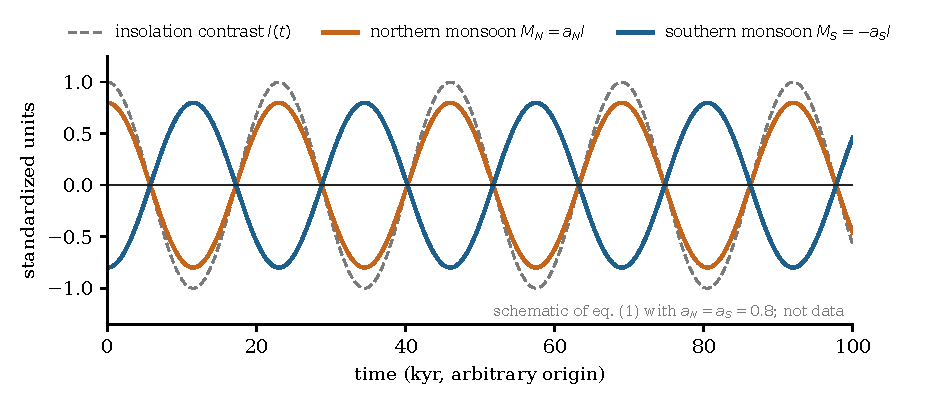
\includegraphics[width=0.95\textwidth]{figures/fig1_orbital_dipole.pdf}
\caption{The idealized orbital dipole of equation~\eqref{eq:linear}. A single insolation contrast $I(t)$ with a period of 23 kyr drives the northern and southern monsoon indices with opposite signs, so that the two curves are exact mirror images. The figure is a schematic generated from the equation with $a_N=a_S=0.8$ and no residual terms. It is not a reconstruction and uses no data from the source record.}
\label{fig:dipole}
\end{figure}

\subsection{Why the dipole is empirically compelling}

The conventional account is not weak, and it should be presented as the strong position it is. \citeauthor{olson2026} take the difference between the standardized Andean and Asian isotope records as a proxy for the strength of the dipole, and they report that this index correlates with the cross-equatorial insolation difference between July at 30$^\circ$N and January at 30$^\circ$S with $r = 0.67$ ($P < 0.001$). The Andean record taken alone correlates more weakly with the summer cross-equatorial insolation gradient ($r = 0.35$), and, to a lesser extent and with the opposite sign, with local summer insolation at 11$^\circ$S ($r = -0.26$). A correlation of 0.67 corresponds, if the relation is treated as linear, to roughly 45 percent of the variance of the dipole index. The orbital account is therefore substantial without being exhaustive, a point that matters for the argument below. The insolation series is computed from orbital mechanics \citep{laskar2004}, the speleothem records are measured in caves on opposite sides of the planet, and the cave chronologies depend on uranium-thorium decay and not on orbital tuning of the climate signal. A correlation between such independently obtained series is difficult to dismiss as an artefact of shared processing.

The relationship is also not an incidental correlation of the kind that two slowly varying quantities can produce by chance, because it follows from physical reasoning that was developed before the long records were available. The theory predicts the sign of the response in each hemisphere, the period at which it should appear, and the approximate timing relative to the forcing. A record that confirms all three has tested a mechanism and not only fitted a curve. For this reason any account of the exceptional events must preserve the explanatory success of the orbital picture. The question is not whether the orbital mechanism operates, since the evidence for it is excellent, but whether its operation is sufficient to determine the observed behaviour under all the conditions the record spans.

The record itself shows where the orbital account strains. Insolation forcing was weakest during Marine Isotope Stage 11, and the authors report that the dipole broke down in that interval, with the two monsoons no longer closely mirroring one another. They note that age uncertainty is greatest in this part of the record, much of which is covered by a single speleothem, so the breakdown may be partly a product of the evidence. They also suggest that the extreme loss of Northern Hemisphere ice during this warm interglacial, combined with a weak cross-equatorial insolation gradient, may have created a climate state in which forcings other than insolation were more dominant over the global monsoon. The suggestion anticipates the argument of the following sections, that the dipole is the dominant response under a range of boundary conditions and not an unconditional law, and it arises in the source paper before any of the synchronous events are considered.

\section{Four Hundred and Fifty Thousand Years in Stalagmite Calcite}

\subsection{Constructing the South American record}

The new record is assembled from stalagmites collected in three caves, Antipayaguna, Pacupahuain, and Huagapo, on the eastern flank of the Peruvian Andes in the upper Amazon Basin. In total, 30 stalagmites contribute to the composite, 23 of them new and seven previously published, and the series rests on 13,939 oxygen-isotope measurements. Chronologies are established by uranium-thorium dating, with 217 new ages obtained for the study and 90 published ages incorporated, and the age model of each stalagmite is built with the Bchron algorithm. The composite extends across approximately 450,000 years with an average temporal resolution of 50 years, which is long enough to span several glacial cycles and many precessional cycles and therefore long enough to ask whether a regularity persists across different climatic backgrounds. Earlier speleothem records from the Southern Hemisphere were limited to the last two ice-age cycles, and the authors describe this record as the first to demonstrate the strength of the interhemispheric monsoon dipole over orbital timescales. Its comparison with the established Asian cave composites is what makes a quantitative statement about the interhemispheric relationship possible.

The measured quantity is the ratio of oxygen isotopes in the calcite, conventionally expressed as $\delta^{18}\mathrm{O}$. The connection to rainfall runs through the fractionation of water isotopes during atmospheric moisture transport. As an air mass moves inland from its oceanic source and loses water as precipitation, the heavier isotopologues condense preferentially, and the remaining vapour, along with later rainfall derived from it, becomes progressively depleted in $^{18}\mathrm{O}$. Under the moisture-transport interpretation adopted for these sites, a stronger monsoon, with more intense upstream rainout along the trajectory, produces rainfall and therefore drip water with lower $\delta^{18}\mathrm{O}$, and this signal is recorded in the calcite that the drip water deposits. Lower values in the calcite are thus read as indicating a stronger monsoon, and higher values a weaker one, which is the sign convention behind the discussion of simultaneous wetting and drying below.

\subsection{The problem of interpreting a proxy}

A proxy is not the physical variable it is used to reconstruct. The oxygen-isotope ratio in speleothem calcite responds to several processes at once. It reflects the isotopic composition of the source water, which depends on conditions in the oceanic region where moisture originates, as well as the degree of upstream rainout, the amount of local precipitation, and the temperature at which the calcite forms. It reflects the mixing and residence time of water in the karst above the cave. Different combinations of these influences can produce the same isotopic value, and the conversion of the isotopic series into a statement about monsoon intensity therefore depends on an interpretive model. The reconstruction is an inference about rainfall, and it inherits the uncertainty of the model that licenses the inference.

The authors address the problem of separating local effects from regional monsoon behaviour by comparison with an independent archive. The Lake Junín glacial index is a sediment-based proxy of glacier extent in the mountains above the caves, drilled about 30 km from them and discussed by \citet{rodbell2022} in the context of 700,000 years of tropical Andean glaciation, and it responds primarily to local temperature and precipitation. After both series are standardized, subtracting the glacial index from the Andean isotope composite is intended to suppress the local component and leave an index of upstream rainout in the Amazon lowlands, which the authors treat as a regional record of South American summer monsoon intensity. The subtraction does not guarantee that result. If the Andean index is $X = aL + bR + \epsilon_X$ and the glacial index is $G = cL + dR + \epsilon_G$, with $L$ a local climate signal and $R$ a regional monsoon signal, then $X - G = (a-c)L + (b-d)R + \epsilon_X - \epsilon_G$, and standardization guarantees neither that $a = c$, which would eliminate the local term, nor that $b \neq d$, which would preserve the regional term. The validity of the correction is therefore supported by the authors' independent comparisons and is not proved by the arithmetic. A principal-component version of the same correction gives a nearly identical result, and the regional index is compared with an independent speleothem record from the western Amazon lowlands spanning the past 250,000 years. Two features of this procedure deserve notice. The first is that the regional index depends on the age model of the Junín record, which has a larger uncertainty than the cave composite, a dependence the authors examine by applying the two-standard-deviation error envelope of the Junín age model. The second is that the synchronous events discussed below are identified from the mean of the Andean composite and the Asian record, not from the Junín-corrected index, so the local signal is argued to be secondary and is not removed from the series on which the events rest. The comparison does not convert any of these records into a direct measurement of rainfall, but it narrows the range of interpretations that remain tenable, and this narrowing is the most that proxy comparison can deliver.

\subsection{Chronology, resolution, and uncertainty}

Two properties of a record are routinely confused and should be kept apart. Sampling resolution is the spacing of the measurements along the record, and it determines the shortest variation that could in principle be resolved. Chronological precision is the uncertainty with which each measurement can be assigned a calendar age, and it determines how reliably one record can be aligned with another. A record can be sampled densely and dated poorly, or the reverse. For a study whose central claim concerns the simultaneity of events in two distant archives, chronological precision is the more consequential property, since an offset of a few centuries in the age model is enough to convert synchronous behaviour into apparent lead or lag, or the reverse.

The composite record has gaps, because individual stalagmites grow intermittently and the intervals during which none was growing are not represented; the authors list six, at roughly 7.0 to 7.7, 98 to 104, 113 to 115, 196 to 203, 231 to 247, and 330 to 371 thousand years before present. Stalagmite ages carry an average uncertainty of about one percent, but the absolute uncertainty grows with age, reaching roughly two thousand years for Marine Isotope Stage 6, and it is largest in Stages 11 and 12, where some portions rest on a single stalagmite. Alignment of independent archives compounds these difficulties, since the Asian and Andean records carry separate age models with separate uncertainties, and the Lake Junín record has its own. More generally, the enterprise illustrates a recurrent problem in the study of dynamical systems from historical traces: the dynamical relationships of interest must be reconstructed from observations that are incomplete, indirect, and imprecisely timed. The remainder of the essay takes the reconstructed history as a serious but fallible representation of past behaviour, and it avoids treating the rainfall history as if it were an instrumental measurement.

\section{Ten Departures from the Dipole}

\subsection{Defining synchronous behaviour}

The identification of departures requires an operational definition of synchronicity. \citeauthor{olson2026} resample the Andean composite and the Asian record to a common 50-year time step, express each in standard-deviation units, and take both the difference and the mean of the two series. The difference serves as the dipole index. The mean serves as an index of synchronicity: when the two records move in opposite directions the mean stays close to zero, and when they move together it departs from zero in the common direction. Intervals in which the mean lies outside plus or minus two standard deviations are designated as extreme synchronous excursions, and adjacent excursions are grouped into events that are classed as wet, dry, or dry during a termination, with events of zero duration excluded. The construction has the useful property that the dipole, which is the dominant mode of variability, cancels in the average, so that what survives is the part of the signal shared by the two hemispheres.

The sign convention explains why a common sign in the isotope records corresponds to simultaneous wetting or drying. Because lower isotope values correspond to stronger monsoon rainfall in both regions, a simultaneous rise in the isotope values of both records indicates simultaneous weakening, and a simultaneous fall indicates simultaneous strengthening. No sign inversion between the two archives is needed, since the isotopic fractionation mechanism operates in the same direction in each. The standardized mean is therefore a physically interpretable measure of whether the two monsoons are, at a given time, jointly stronger or jointly weaker than their long-term averages.

Figure~\ref{fig:record} plots the composite record as tabulated in the supplementary data of \citeauthor{olson2026}, together with the rolling Pearson correlation between the Andean and Asian records, computed over a window of about ten thousand years (40 points at 250-year spacing). The Asian record is not part of that table, so the figure shows the correlation as supplied and not the synchronicity index itself. The correlation is negative in 64 percent of the 1,489 windows for which it is defined, and significantly negative (at $p<0.05$ under the Ebisuzaki test) in 11 percent, which is the quantitative content of the statement that the two monsoons are antiphased most of the time. It is positive in 36 percent of windows, but positive and significant in fewer than 5 percent, and those windows cluster around Terminations II, III, and V, with a smaller cluster near 397 thousand years before present. The window around Termination I is positive but does not reach significance. These percentages describe how prevalent each correlation pattern is along the sampled timeline. They are not frequencies of independent climatic states, because windows advanced by 250 years share about 97.5 percent of their span with the preceding window, so that the record holds roughly 45 non-overlapping ten-thousand-year windows and not 1,489 independent tests. The per-window significance also differs from the significance of the clustering of positive windows near terminations, which would need its own null hypothesis and test and is not attempted here. The dominance of antiphase and the clustering of the exceptions in particular intervals are both visible before any threshold is applied.

\begin{figure}[!htbp]
\centering
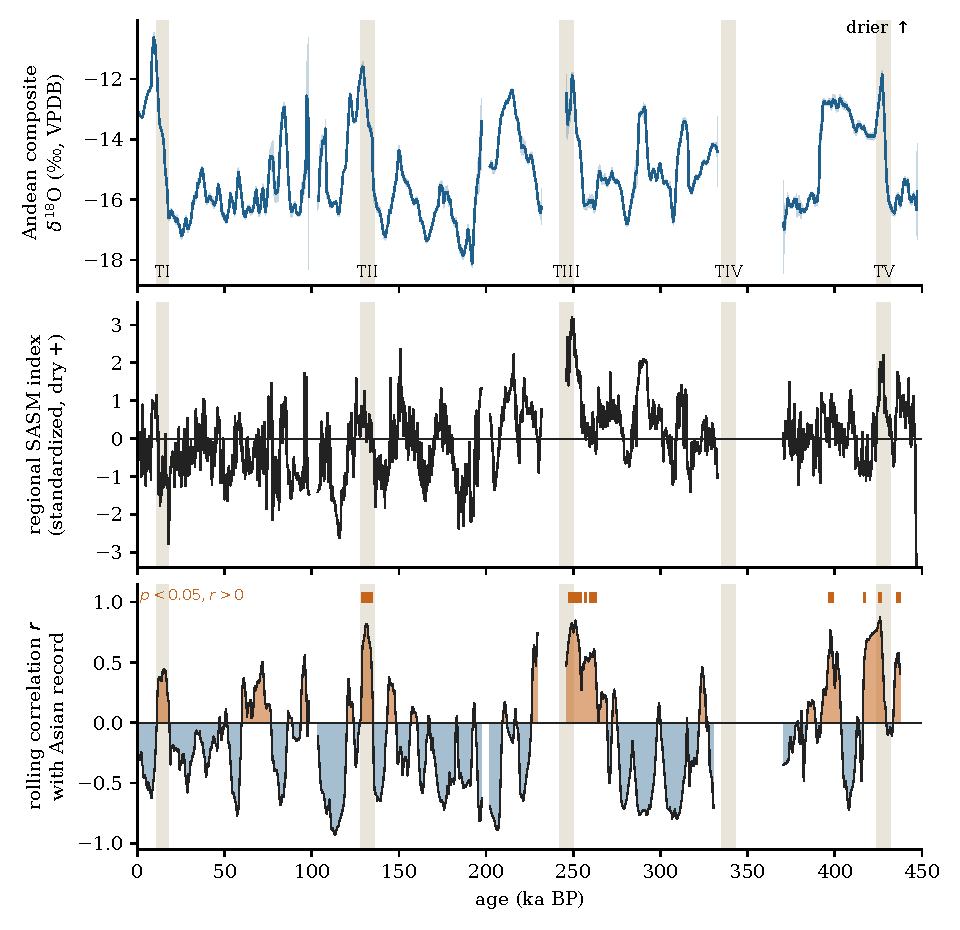
\includegraphics[width=0.98\textwidth]{figures/fig4_record.pdf}
\caption{The Andean composite record and its relation to the Asian monsoon, plotted from Supplementary Table 3 of \citet{olson2026} in 250-year bins. (a) Composite stalagmite $\delta^{18}$O with its 95 percent confidence interval; higher values indicate a drier monsoon. (b) The regional South American summer monsoon index, the standardized Andean composite minus the standardized Lake Jun\'in glacial index; the final value at 447 ka falls outside the plotted range. (c) Rolling Pearson correlation between the Andean and Asian records, with ticks marking windows that are positive and significant at $p<0.05$ under the Ebisuzaki phase-randomization test. Gaps are intervals in which no stalagmite was growing, and missing values are left as gaps and not interpolated. The confidence interval in (a) and the correlations and $p$ values in (c) are the columns supplied in the table and were not recomputed, and each rolling window is placed at the age tabulated for it. The percentages quoted in the text were counted by the author from those columns over the 1,489 bins for which a correlation is supplied (script \texttt{fig4.py}). Shaded bars are approximate termination windows drawn by the present author after the grey bars in the source figures, not values taken from the paper.}
\label{fig:record}
\end{figure}

\subsection{Simultaneous weakening in warm and warming intervals}

The ten events differ in sign and in the climatic conditions under which they occurred. The article distinguishes dry events that accompany glacial terminations, the rapid transitions from full glacial to interglacial conditions, from four dry events that occur within interglacial intervals, and from two wet events that fall in Marine Isotope Stage 6. The synchronous weakenings that accompany terminations recur with the periodicity of the glacial cycle, about 100,000 years, and they coincide with major increases in atmospheric carbon dioxide and global temperature, which were intervals of reduced meridional temperature gradient. The accompanying research briefing, by \citet{rodbellolson2026}, reports that during periods of rapid warming or warmth the two monsoon systems weakened synchronously for 100 to 4,250 years. The breadth of this range indicates that the phenomenon is not a single stereotyped event but a class of episodes that may differ in mechanism as well as in length. Termination I stands somewhat apart. Heinrich event 1 interrupted that termination and produced a major wet pulse in the South American record, so that the two monsoons remained anticorrelated over the precessional cycle, and the weakening associated with it is less pronounced than in earlier terminations.

The forcing configuration during the other terminations is itself informative. Cross-equatorial insolation is near neutral and rising toward the Northern Hemisphere, conditions that should strengthen the Asian monsoon and weaken the South American. The South American monsoon is weak, as expected, but it is the Asian monsoon that behaves anomalously. An ITCZ reconstruction from the Cariaco Basin places the Atlantic ITCZ near its neutral position, not displaced to the south, while North Atlantic sea surface temperatures are cool, atmospheric carbon dioxide is high, and the cross-equatorial temperature gradient is weak. The authors conclude that this combination dampened the global monsoon. The result bears directly on the earlier proposal of \citet{cheng2016} that weak monsoon intervals were triggered by a southward ITCZ deflection, since a southward migration of the monsoon belt should have strengthened the southern monsoon systems, and the record shows that it did not.

The association with terminations is suggestive without being conclusive. Terminations are the intervals of fastest and most coordinated change in the climate system, and almost every climatic variable is changing at once. A statistical association between an anomaly and a termination is therefore expected under many different mechanisms, a point that returns in Section~VIII. What the association does establish is that the departures are not randomly distributed through the record, and that they cluster under conditions in which the boundary conditions of the ocean, the atmosphere, and the cryosphere are being rapidly rearranged.

The four dry events that occur within interglacial intervals have a different structure. There the cross-equatorial insolation gradient strongly favours the Southern Hemisphere monsoon, at about minus one standard deviation, and it is the South American monsoon that behaves anomalously by remaining weak. The ITCZ is held near the equator, at about plus 0.1 standard deviations, by anomalously warm North Atlantic sea surface temperatures, at about plus 0.7 standard deviations, which the authors describe as impeding the development of the South American monsoon and compare to the Dansgaard-Oeschger events of the last glacial cycle. The interglacial and termination dry events share high carbon dioxide and a near-neutral ITCZ, and the authors observe that all other forcing factors are opposite, so that interhemispheric weakening can arise under both interglacial and transient termination boundary conditions.

\subsection{Simultaneous strengthening under glacial conditions}

The record also contains synchronous wet events, which the article places only in Marine Isotope Stage 6, the glacial interval preceding the last interglacial, where two simultaneous extreme wet events are marked. The accompanying briefing describes joint strengthening during four intervals of especially cold global conditions, with a mean duration of about 2,000 years. The main article identifies two such events in Marine Isotope Stage 6, whereas the briefing refers to four intervals, and neither source as available for this essay states how the two enumerations are reconciled. The difference requires clarification from the underlying event definitions or the supplementary tables, and it is left unresolved here. The essay follows the article in treating the wet events as belonging to the penultimate glacial, and nothing in the argument depends on the count. These events must be distinguished from the dry anomalies. They occur under cold and ice-dominated conditions, whereas the dry anomalies cluster in warm or warming conditions, and it would be a mistake to treat the two classes as mirror images produced by a single mechanism with opposite sign. During the wet events the insolation gradient favours the Northern Hemisphere monsoon, yet the South American monsoon is also strong. The authors suggest that anomalously cold North Atlantic sea surface temperatures, below minus 0.5 standard deviations, and a southerly ITCZ position may explain these brief intervals of strong South American monsoon, and they compare the events to the Heinrich events of the last glacial cycle. The existence of anomalies of both signs argues against any explanation which attributes departures from the dipole solely to warming, since the departures occur under both warm and cold boundary conditions. It also suggests that what the departures share is not a particular climatic state but the circumstance that some influence other than the interhemispheric insolation contrast has become strong enough to override or add to the orbital response in both regions at once.

\subsection{The meaning of synchronicity}

The word synchronicity invites a misreading that the physics does not support. In the theory of coupled oscillators, synchronization denotes a specific dynamical condition, in which interacting systems adjust their rhythms through mutual coupling until they become phase-locked \citep[see][]{pikovsky2001}. Two systems can, however, show simultaneous anomalies without being synchronized in this sense. If both are driven by a common external influence, each will respond at the same time, and the coincidence of the responses reflects the shared forcing and not any coupling between the systems. The distinction is practical as well as semantic. Synchronization by coupling implies that the systems influence one another and that disturbing one will disturb the other, whereas common driving implies no such mutual dependence.

For the monsoon events, the available observations do not discriminate between these cases, and a further set of questions follows. The exceptional events might represent a failure of the orbital response, in which the mechanism that normally generates the dipole ceased to operate. They might represent the superposition of an additional response upon an orbital response that continued unchanged. They might represent a change in the coupling structure of the system, so that the same forcing produced a different pattern of response. These three readings have different implications and they are carried through the following sections, with the proposition that the orbital mechanism may have remained physically operative throughout, while its consequences were obscured by something else, given particular attention.

The authors describe the events as in-phase responses to a shared set of forcing conditions that includes a neutral ITCZ and anomalous North Atlantic temperatures, and they conclude that the global monsoon can reorganize itself during intervals of rapidly changing boundary conditions. The verb is used descriptively, and the article does not claim that a stability threshold was crossed. It is also notable that in the termination events the Asian monsoon is the one behaving anomalously relative to insolation, whereas in the interglacial dry events and the glacial wet events it is the South American monsoon, so the departures are not a uniform failure of one hemisphere's response.

\section{Redistribution Is Not Conservation}

A simplified reading of the monsoon dipole runs as follows. Under the influence of differential heating, the ITCZ shifts toward one hemisphere, and rainfall that would have fallen in the other hemisphere falls instead in the first. The rain belt moves, rainfall is transferred, and one monsoon gains what the other loses. The physical theory of ITCZ displacement does not make this claim in so literal a form. It concerns changes in the atmospheric transport of energy, in tropical circulation, and in the geographical distribution of precipitation, and these mechanisms can generate an approximate dipole without implying exact compensation between any two regions. The literal reading is nevertheless a natural shorthand, and on that picture a simultaneous weakening of both monsoons appears paradoxical, since it seems to require that rainfall disappear from the system. The paradox dissolves once it is recognized that the shorthand rests on an unjustified step, from the redistribution of rainfall by a shifting circulation to the conservation of rainfall between two chosen regions. The argument is thus directed at a displacement-only approximation and not at the physics of ITCZ migration.

The relevant physical constraint is the atmospheric moisture budget. For the column-integrated water vapour $W$, the budget reads
\begin{equation}
\frac{\partial W}{\partial t} + \nabla\cdot\bQ = E - P,
\label{eq:budget}
\end{equation}
where $\bQ$ is the vertically integrated horizontal moisture flux, $E$ is evaporation from the surface, and $P$ is precipitation. Averaged over a long interval, the storage term is small, and the budget states that precipitation exceeds evaporation where the moisture flux converges and falls short of evaporation where it diverges. This is a statement of local conservation of atmospheric water. It constrains how precipitation, evaporation, and moisture transport can vary together at each point, but it places no constraint on the sum of precipitation anomalies over two particular regions, because the water balance of each region includes terms that are free to change. Precipitation in a monsoon region can fall because the moisture flux converging on it weakens, because evaporation from the sources that supply it declines, because the circulation that delivers moisture is rerouted toward some third region, or because the vertical structure of the atmosphere suppresses convection despite adequate moisture. Any of these can happen in both hemispheres simultaneously without violating equation~\eqref{eq:budget}.

Three propositions are therefore easily confused and should be separated. The first is that atmospheric water obeys a conservation equation. This is a general physical constraint and it is never violated. The second is that precipitation is redistributed geographically as circulation shifts, which is true of many circulation changes and describes a common mechanism, but is not a law. The third is that the sum of the rainfall anomalies in two selected regions is constant, so that a loss in one is balanced by a gain in the other. Of the three, only the first is a general physical constraint. The third would hold only if the two regions together exhausted the relevant moisture budget and if no other region or process could absorb the change, and neither condition has a basis in the physics.

The dipole is accordingly an emergent response pattern and not a conserved quantity. It is what the coupled system produces when the dominant influence is the interhemispheric insolation contrast and the remaining boundary conditions are in a range in which that influence determines the position and strength of the rain belts. Under other conditions the same equations admit other patterns. This reading replaces the misleading interpretation that the synchronous events somehow violate the expected physics. They violate a simplified model of the physics, in which a conservation law for the atmospheric water budget was silently promoted to a conservation law for regional rainfall. The physics itself was not suspended, and the right response to the anomalies is therefore to ask which additional terms in the full budget became large, and not to search for a failure of the conservation principle.

The source paper supplies a concrete instance of this reasoning. In freshwater-hosing experiments from the North Atlantic Hosing Model Intercomparison Project, a weakened overturning cools the North Atlantic and warms the tropical South Atlantic, where convection intensifies and compensating subsidence is induced over the southeastern equatorial Pacific through a Walker circulation anomaly. The most pronounced circulation anomalies are declines in the strength of the South Atlantic and Indian subtropical highs, both of which are integral to the South American and Asian monsoon circulations. The four models analysed by \citeauthor{olson2026} show pronounced drying at the locations of both the Andean and the Asian cave sites in the peak rainy season. The moisture budget of equation~\eqref{eq:budget} holds in these experiments as it does anywhere, and the simultaneous drying reflects changes in the moisture flux and in the circulation that organizes it.

\section{Oceanic Teleconnections and Conditional Coupling}

\subsection{The Atlantic meridional overturning circulation}

The extratropical ocean enters the argument through its capacity to alter the tropical atmosphere at a distance. The Atlantic meridional overturning circulation (AMOC) carries heat northward across the equator in the Atlantic, so that the Northern Hemisphere is warmer than it would otherwise be relative to the Southern. Freshwater delivered to the North Atlantic, for example by the melting of ice sheets during a deglaciation, reduces the density of surface waters, can weaken the overturning, and reduces the northward ocean heat transport. The resulting cooling of the North Atlantic increases the interhemispheric temperature contrast in favour of the south, and atmospheric energy-budget arguments predict a southward displacement of the ITCZ \citep{schneider2014}. On this account \citet{cheng2016} hypothesized that the weak monsoon intervals of the Asian record during terminations were triggered by a southward ITCZ deflection, with heat pooling in the equatorial Atlantic, which weakened the northern monsoon and strengthened the southern. Such a redistribution account makes a testable prediction about the South American record, namely that the southern monsoon should strengthen when the Asian monsoon weakens.

The record of \citeauthor{olson2026} does not bear out that prediction. The South American monsoon is weak during the termination events, in step with the Asian monsoon, and the Cariaco Basin ITCZ reconstruction places the Atlantic ITCZ near its neutral position during those intervals and not displaced to the south. The authors point instead to the combination of a weak cross-equatorial temperature gradient, cool North Atlantic sea surface temperatures, and high carbon dioxide. The AMOC mechanism therefore remains a plausible contributor to simultaneous weakening, but its route to the monsoons is not a simple migration of the rain belt. Multi-model hosing experiments of the kind assembled by \citet{benyami2024}, re-analysed by \citeauthor{olson2026} for four models, show a heterogeneous South American response: parts of the southeastern Andes and central-eastern Brazil become wetter while the northern monsoon regions near the equator become drier, a pattern the authors compare with South American records from Heinrich event 1. The effect of an AMOC weakening on a given monsoon is therefore conditional on the other components of the system. The magnitude and geographical expression of the ITCZ displacement that a weakened overturning produces are themselves state dependent, varying with background ocean temperatures, ice-sheet geometry, seasonality, and the structure of the atmospheric circulation, so the chain from freshwater input to regional rainfall should not be read as a deterministic sequence that holds identically across climatic states.

\subsection{The Pacific Walker Circulation}

A second pathway runs through the tropical Pacific, and it is useful to separate what is inferred from the proxy records, what is obtained from climate models, and what is proposed as the mechanism connecting the two. The Walker Circulation is the zonal overturning of the tropical atmosphere, with rising air over the warm western Pacific and sinking air over the cooler eastern Pacific, sustained by the east--west gradient of sea surface temperature.

The proxy evidence is limited. The zonal sea surface temperature gradient, defined as eastern minus western Pacific and estimated from two marine cores, is slightly positive at the times of the termination events, the sign analogous to the El Ni\~no phase of the El Ni\~no--Southern Oscillation. This is an observation about surface temperature at two locations. It does not establish the atmospheric circulation that prevailed during an ancient event.

The mechanism comes from modern and model-based studies, and \citeauthor{olson2026} present it as a proposal. They argue that the Pacific Walker Circulation may link the North Atlantic to the global monsoon: cooling of the North Atlantic suppresses convection there and shifts the Walker cells, displacing rainfall toward the Pacific in what has been called a trans-basin interaction, and the resulting weakening of the Walker Circulation has been linked to a reduced Asian monsoon both today and in palaeoclimate records. As the eastern Pacific warms, the location of convection shifts and a tropical Rossby-wave response develops, with twin anticyclones around the equator, which reorganizes upper-level flow, suppresses convection over the northern Amazon, and reduces rainfall across tropical South America.

The proxy gradient is consistent with this pathway, and the hosing experiments described in Section~V show a circulation response of the right kind, but the two have not been joined into a reconstruction of the events themselves. If the pathway operates, a reorganization of the Pacific gradient can weaken the South American monsoon regardless of what is happening in the Atlantic and regardless of the orbital configuration.

The wider lesson is that changes in one ocean basin can influence rainfall in geographically distant monsoon regions, and that a given monsoon is exposed to several basins at once. The Asian monsoon is influenced by the Indian and western Pacific oceans and by the state of the high-latitude north. The South American monsoon is influenced by the tropical Atlantic and by the equatorial Pacific. When a single global disturbance, such as the transition out of a glacial state, changes several of these basins together, both monsoons can be pushed in the same direction by different routes. The synchronous weakening observed during terminations does not require a single mechanism connecting the two regions. It requires only that the processes acting on each region happen to be activated by the same large-scale transition. \citeauthor{olson2026} suggest in this vein that the Pacific zonal gradient may help synchronize the two systems during terminations, while noting that the connection between Atlantic sea surface temperatures and the Asian monsoon has been a subject of debate.

\subsection{Boundary conditions as dynamical variables}

These considerations suggest a formal distinction. A response function with fixed parameters has the form
\begin{equation}
\bM = F(\bI;\theta),
\label{eq:fixed}
\end{equation}
where $\bM$ collects the monsoon responses, $\bI$ the orbital forcing, and $\theta$ is a set of constant parameters. Equation~\eqref{eq:linear} is of this kind. A state-dependent response has parameters that themselves depend on the climatic state,
\begin{equation}
\bM = F\bigl(\bI;\theta(\bB)\bigr),
\label{eq:state}
\end{equation}
where $\bB$ denotes the relevant oceanic, cryospheric, and atmospheric boundary conditions, including the strength of the overturning circulation, the Pacific temperature gradient, the extent of the ice sheets, and the concentration of greenhouse gases. In the fixed-parameter case, one orbital configuration produces one monsoon response whatever the other conditions. In the state-dependent case the same orbital configuration can produce different responses depending on $\bB$.

The boundary conditions are not external settings that experimenters choose. They are themselves components of the climate system, and they evolve in response to its dynamics, sometimes on the same timescales as the monsoons and sometimes much more slowly. The distinction between forcing and boundary condition is accordingly one of timescale and of convenience, and not an absolute division. The argument that follows is not merely that the climate has many causes, which is both true and uninformative. It is that the relative influence of those causes changes with the state of the system. In a regime in which the interhemispheric insolation contrast dominates the energy budget of the tropics, the dipole is a good description. In a regime in which another influence has become comparable, the dipole may be partly or wholly masked, and the same orbital forcing continues to act but no longer dominates what is observed.

A distinction is needed here between state-dependent coupling and nonlinear dynamics, because the two are easily blurred. A model whose coefficients vary with the boundary conditions can remain linear in its state variables. For example, $\dot C = -\lambda_C(\bB(t))\,C + f(t)$ is a linear, time-varying differential equation in $C$ when $\bB(t)$ and $f(t)$ are prescribed, and it has neither multiple equilibria nor a bifurcation. If $\bB$ in turn evolves as a function of $C$, the complete coupled system may be nonlinear even though the equation for $C$ taken alone is linear. The hierarchy matters for what follows. The observations require at most a forced or a conditional response and do not require nonlinear internal dynamics, so the strongest conclusion the evidence supports is conditional response and not nonlinearity itself.

\section{Common Modes, Difference Modes, and Dynamical Reorganization}

This section develops a mathematical interpretation that is the author's own. It is not drawn from the analysis performed by \citeauthor{olson2026}, and the equations below are idealizations introduced to clarify what different explanations would imply. They are not fitted to the data and no claim is made that the actual monsoon system obeys them.

\subsection{Decomposing interhemispheric variability}

Let $x_N$ and $x_S$ be rainfall-oriented standardized anomalies for the northern and southern monsoon records, oriented so that positive values correspond to wetter conditions. Define the difference mode and the common mode,
\begin{equation}
D = \frac{x_N - x_S}{2}, \qquad C = \frac{x_N + x_S}{2}.
\label{eq:modes}
\end{equation}
The difference mode describes interhemispheric opposition and the common mode describes simultaneous variation. The transformation is invertible, and the original anomalies are recovered as
\begin{equation}
x_N = C + D, \qquad x_S = C - D.
\label{eq:inverse}
\end{equation}
The decomposition makes it possible to distinguish orbital dipole behaviour from common forcing. If the orbital response is a pure dipole, in the sense that the two hemispheres respond with equal and opposite amplitudes, it projects entirely onto $D$ and leaves $C$ unaffected; the case of unequal amplitudes is treated below. An influence that raises or lowers both monsoons together projects onto $C$. A weakening of both monsoons is then a large negative excursion of $C$, and it is compatible with an undiminished $D$: the two monsoons can both be anomalously dry while the difference between them continues to follow the orbital contrast. In this representation the synchronous events appear as excursions along a direction orthogonal to the one the orbital forcing excites, and not as contradictions of the orbital response. A numerical example shows the point. If $C = -2$ and $D = 0.5$, then $x_N = -1.5$ and $x_S = -2.5$: both hemispheres are anomalously dry, yet the difference mode is nonzero and the northern monsoon remains wetter than the southern by one standardized unit. Simultaneous negative anomalies do not imply that the difference mode has vanished.

The source paper works with isotope anomalies in which larger values indicate drier conditions, and it defines its dipole index as the Andean minus the Asian standardized record and its synchronicity index as their mean. With the Asian record taken as the northern series and the Andean record as the southern, and with the anomalies sign-reversed to be rainfall oriented, its difference is $2D$ and its mean is $-C$. The detection procedure is therefore a thresholding of the common mode at plus or minus two standard deviations, and the decomposition introduces no new data. What it contributes is a framework in which the three possible explanations of the events can be stated as claims about the dynamics of $C$ and $D$ separately.

The statement that an orbital response projects entirely onto $D$ holds only under a symmetric-response assumption. Let the hemispheric responses to the insolation contrast $I$ be
\begin{equation}
\begin{split}
x_N &= a_N(\bB)\,I + g_N(\bB),\\
x_S &= -a_S(\bB)\,I + g_S(\bB),
\end{split}
\label{eq:asym}
\end{equation}
where $g_N$ and $g_S$ collect everything not driven by the orbital contrast. The modes are then
\begin{equation}
D = \frac{a_N + a_S}{2}\,I + \frac{g_N - g_S}{2}, \qquad
C = \frac{a_N - a_S}{2}\,I + \frac{g_N + g_S}{2}.
\label{eq:asymmodes}
\end{equation}
Two consequences follow. First, a common-mode response can arise even in a static model that is linear in the insolation, because the orbital forcing itself projects onto $C$ whenever $a_N \neq a_S$. Second, if the sensitivities depend on the boundary conditions, so that $a_N - a_S$ changes with $\bB$, then the weight with which the same insolation contrast enters the common mode changes with the climatic state. This is the simplest form of state-dependent coupling, and it requires no nonlinear dynamics. Because $I$ oscillates at the precessional period, however, the term $(a_N - a_S)I/2$ by itself produces a periodic common-mode signal and not an isolated excursion. Unequal sensitivities change what the orbital forcing contributes to $C$, but the remainder of an event would have to come from the term $(g_N + g_S)/2$ or from a time-dependent change in $\bB$.

\subsection{A minimal state-dependent model}

A minimal model with this structure is
\begin{equation}
\dot D = -\lambda_D D + a I(t) + \eta_D, \qquad
\dot C = -\lambda_C(\bB) C + f(\bB, I) + \eta_C,
\label{eq:minimal}
\end{equation}
in which $\lambda_D$ and $\lambda_C$ are relaxation coefficients, $a$ is the orbital response coefficient, $f$ is a forcing term in the common mode that may depend on the boundary conditions and on the insolation, and $\eta_D$ and $\eta_C$ are noise terms representing unresolved variability. The relaxation coefficient measures how quickly a mode returns toward equilibrium after a disturbance. The interpretation is that the difference mode is strongly slaved to the orbital forcing, with $\lambda_D$ fixed, while the common mode has a relaxation rate that depends on the state of the system, so that its susceptibility to forcing and the duration of its excursions can change as the boundary conditions change.

Two qualifications attach to this model. The first concerns units. If $C$ and $D$ are dimensionless standardized anomalies and time is measured in kiloyears, then $\lambda_D$ and $\lambda_C$ are in inverse kiloyears, and $aI$, $f$, and the noise terms must carry units of standardized anomaly per kiloyear. The second is more substantive. Writing separate equations for $C$ and $D$ is a modelling assumption and not a consequence of the decomposition, because an invertible change of coordinates does not make the transformed variables evolve independently. Suppose the hemispheric anomalies obey $\dot{\mathbf{x}} = A\mathbf{x} + \mathbf{u}$ with $A = \begin{pmatrix} p & q \\ r & s \end{pmatrix}$, and let $\mathbf{z} = (C, D)^{\top} = T\mathbf{x}$ with $T = \tfrac12\begin{pmatrix} 1 & 1 \\ 1 & -1 \end{pmatrix}$. Then $\dot{\mathbf{z}} = TAT^{-1}\mathbf{z} + T\mathbf{u}$, and the off-diagonal entries of $TAT^{-1}$ are $\tfrac12(p - q + r - s)$, which couples $D$ into $C$, and $\tfrac12(p + q - r - s)$, which couples $C$ into $D$. Both vanish when the two row sums of $A$ are equal and the two column sums are equal, which is guaranteed if the two hemispheres have symmetric dynamics, $p = s$ and $q = r$. Asymmetries between the hemispheres, such as the unequal distribution of land and ice, generate coupling between the modes. Equation~\eqref{eq:minimal} should therefore be read as an idealization that neglects this coupling, retained here because it isolates the question of interest and not because it is implied by the hemispheric structure of the system.

A common-mode excursion can occur in this model without eliminating the difference mode. If $f$ becomes large and negative, because for instance an AMOC weakening and a reorganization of the Pacific gradient both suppress rainfall, then $C$ departs from zero and relaxes slowly if $\lambda_C$ is small. During this time $D$ continues to evolve under $aI(t)$ and the dipole is preserved as a pattern superimposed on the common shift. If, in addition, the departures in $C$ are large compared with the amplitude of $D$, the two monsoons will both be dry even though their difference still tracks the orbital contrast. The model thus shows how the same orbital response can persist while the sign of one or both monsoon anomalies is dictated by the common mode. Figure~\ref{fig:modes} shows the behaviour in a numerical integration of equation~\eqref{eq:minimal}.

\begin{figure}[!htbp]
\centering
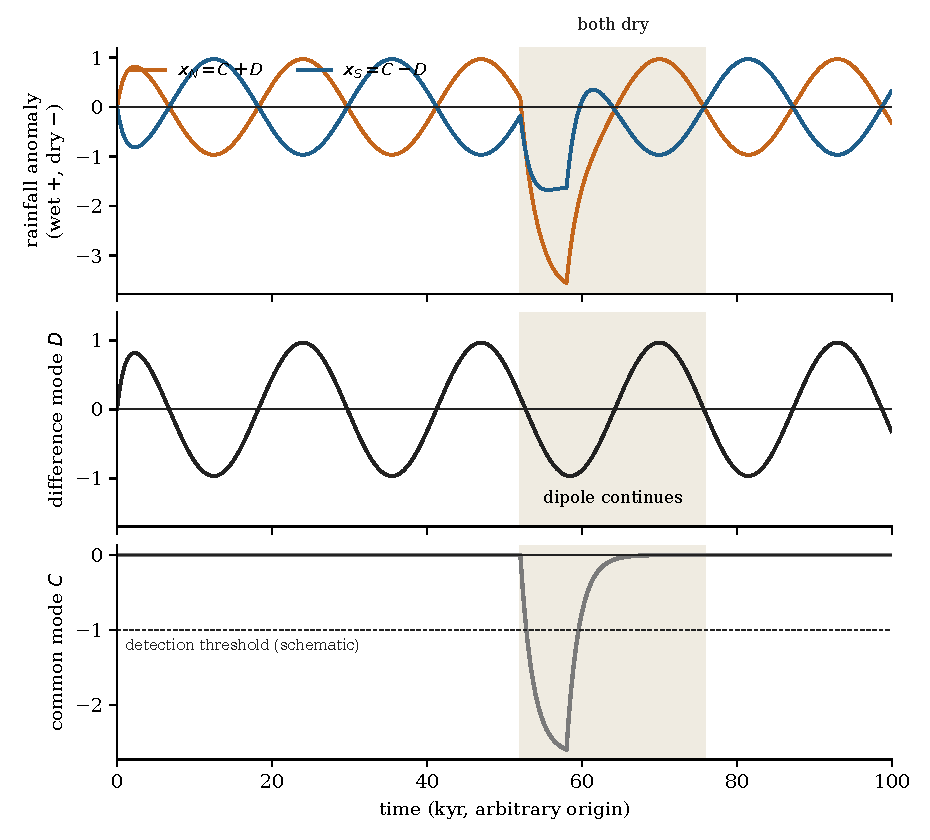
\includegraphics[width=0.95\textwidth]{figures/fig2_common_difference.pdf}
\caption{A common-mode excursion superimposed on an undiminished dipole. The difference mode $D$ is driven by a 23 kyr orbital term, and the common mode $C$ receives a single negative forcing pulse between 52 and 58 kyr. Rainfall anomalies are recovered as $x_N=C+D$ and $x_S=C-D$, so both hemispheres are dry during the shaded interval while $D$ continues to oscillate. Equation~\eqref{eq:minimal} is integrated by the forward Euler method with a step of 0.05 kyr from $C=D=0$ at 0 kyr, using $I(t)=\cos(2\pi t/23)$, $\lambda_D=1$, $\lambda_C=0.6$ and $a=1$ (all per kyr, with $C$ and $D$ in dimensionless standardized units), $f=-1.6$ per kyr for $52<t<58$ kyr and zero otherwise, and no noise terms. The plotted $D$ is the unmodified solution. The shaded interval is placed by eye. The figure is a schematic illustration of the model, not a fit, and the threshold line is placed for illustration only.}
\label{fig:modes}
\end{figure}

\subsection{Nonlinearity and alternative stable configurations}

The model above is linear in $C$ and so has a single equilibrium for any given forcing. Nonlinear dynamics permit richer behaviour. As an illustration, consider
\begin{equation}
\dot C = \mu(\bB)\,C - \beta C^3 + h(t), \qquad \beta > 0,
\label{eq:cubic}
\end{equation}
where $\mu(\bB)$ is a state-dependent linear growth rate, $\beta$ is a cubic saturation coefficient, and $h(t)$ is an external perturbation. Consider first the unforced case $h = 0$. The equilibria satisfy $C(\mu - \beta C^2) = 0$. For $\mu \le 0$ the only real equilibrium is $C = 0$. It is stable for $\mu < 0$ by linearization, since the derivative of the right-hand side there is $\mu < 0$. At $\mu = 0$ the linearization is degenerate, but the origin remains asymptotically stable because $\dot C = -\beta C^3$ there; the stability is nonhyperbolic, and the relaxation is algebraic and not exponential. For $\mu > 0$ there are three equilibria, $C = 0$ and $C = \pm\sqrt{\mu/\beta}$. Linearizing about each shows that the origin is unstable, since the derivative of the right-hand side there is $\mu > 0$, and that the two nonzero equilibria are stable, since the derivative at $C = \pm\sqrt{\mu/\beta}$ is $\mu - 3\mu = -2\mu < 0$. The system therefore passes through a pitchfork bifurcation at $\mu = 0$: a single stable state gives way to two stable states, and a small perturbation that breaks the symmetry selects one of them.

With a nonzero constant perturbation $h$, the bistability persists only within a bounded range. Write $g(C) = \mu C - \beta C^3$ for the unforced part of the right-hand side, so that equilibria under a constant perturbation satisfy $g(C) = -h$. Since $g'(C) = \mu - 3\beta C^2$ and $g''(C) = -6\beta C$, the function $g$ has a local maximum of $+2\mu^{3/2}/(3\sqrt{3\beta})$ at $C = +\sqrt{\mu/(3\beta)}$ and a local minimum of $-2\mu^{3/2}/(3\sqrt{3\beta})$ at $C = -\sqrt{\mu/(3\beta)}$. The line $g = -h$ therefore meets the graph of $g$ three times only while $|h| < 2\mu^{3/2}/(3\sqrt{3\beta})$. When $|h|$ exceeds this value a stable and an unstable equilibrium merge and vanish in a saddle-node bifurcation, so that a system resting on that branch is forced onto the remaining one. This structure is the standard one for the discussion of critical transitions and tipping elements in the climate system, as reviewed by \citet{lenton2008} and by \citet{scheffer2009}. In such systems a slow change in a control parameter, here $\mu(\bB)$, can bring the system to a point at which a small perturbation produces a large and persistent change of state. Figure~\ref{fig:bifurcation} shows both structures. The hysteresis in panel (b) is the quasistatic equilibrium construction: it arises when $h$ varies slowly enough for the state to follow the stable branches and is cycled far enough to cross both folds. A smaller excursion confined to one branch produces no loop, and forcing at a finite rate introduces dynamical delays that are distinct from equilibrium hysteresis.

\begin{figure}[!htbp]
\centering
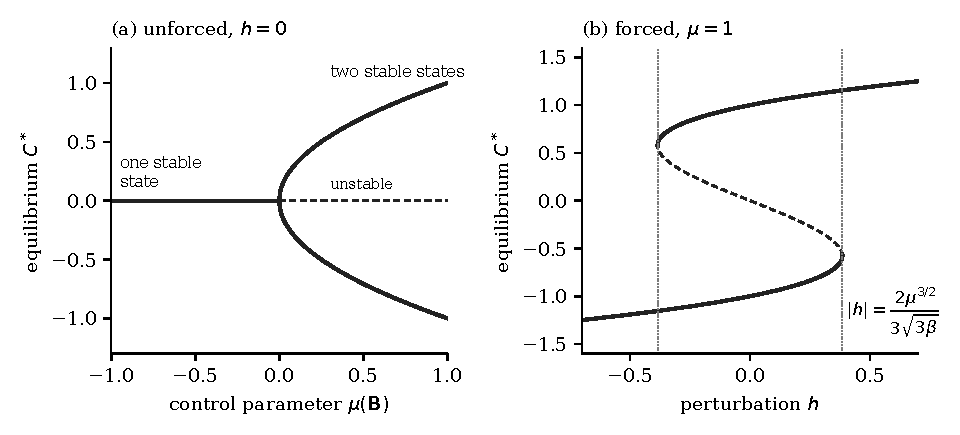
\includegraphics[width=0.98\textwidth]{figures/fig3_bifurcation.pdf}
\caption{Equilibria of the cubic model, equation~\eqref{eq:cubic}, with $\beta=1$. Solid lines mark stable equilibria and dashed lines unstable ones. (a) With no perturbation, a single stable state gives way to two stable states at $\mu=0$ in a pitchfork bifurcation. (b) At $\mu=1$, a slowly varying perturbation $h$ moves the system along one branch until it reaches a fold at $|h|=2\mu^{3/2}/(3\sqrt{3\beta})$, where that branch disappears and the system jumps to the other. If $h$ is cycled far enough to cross both folds, the return path differs from the outgoing path. The curves are quasistatic equilibria computed from $-(\mu C-\beta C^3)=h$, not simulated trajectories. The model is a candidate illustration and carries no claim about the monsoon system.}
\label{fig:bifurcation}
\end{figure}

It must be emphasized that equation~\eqref{eq:cubic} is a candidate model and not evidence that the actual monsoon system crossed a bifurcation. Its function is to show that a mathematically coherent mechanism exists by which a boundary condition acting through $\mu$ could convert a stable common mode into a pair of alternative states, and to specify what such a mechanism would predict. The existence of the model is not evidence for the mechanism, and the data considered in this essay do not demonstrate that any bifurcation occurred.

\subsection{Three explanations of the observed events}

Three explanations of the synchronous events can now be stated in the language of the common mode. The first is a forced common-mode excursion. In this reading the dynamics of $C$ are unchanged, and an additional external influence $f$ or $h$ pushed the system away from its usual state for a period determined by the original relaxation rate. The orbital response is intact, the coupling structure is unchanged, and the events are the transient response to an additional forcing, such as the freshwater input of a deglaciation.

The second is state-dependent coupling. In this reading the relaxation rate $\lambda_C$, the response coefficients, or the forcing term depend on $\bB$, and the events occur because the boundary conditions during a termination placed the system in a configuration of higher susceptibility. The same perturbation applied under different boundary conditions would have produced a smaller or opposite response. This is the interpretation developed in Section~VI. It differs from the first in that the events reflect a change in how the system responds and not only a change in what is applied to it.

The third is a genuine regime transition. In this reading the system crossed a stability threshold, as in the cubic model, and settled for a time into a different configuration whose persistence reflects the stability of that configuration and not the duration of the perturbation that triggered it. This is the strongest of the three claims, and it makes the most specific predictions. It is also the one for which the present evidence is weakest, and the evidential bar for it should be correspondingly high.

The three readings predict different observable signatures. Under a forced excursion, the duration of an event should track the duration and magnitude of the forcing and the recovery should follow the original relaxation time. Under state-dependent coupling, the response to comparable forcing should differ across intervals with different boundary conditions, so that estimated response coefficients should shift systematically. Under a regime transition produced by loss of stability, as in the cubic model, hysteresis and critical slowing down are possible discriminating signatures: the system need not return along the path by which it departed, the approach to a threshold can appear as increasing autocorrelation and variance \citep{scheffer2009}, and the recovery time should be controlled by the stability of the new state. These are signatures of particular dynamical mechanisms and not necessary properties of every regime transition. Noise-induced switching between existing attractors, rate-induced tipping, and some abrupt externally forced changes need not show them, and where they are expected, observed trends in variance and autocorrelation can be confounded by changing forcing, nonstationarity, and proxy uncertainty. No single feature is decisive, and none of these signatures should be assumed in advance. Each explanation should be treated as a hypothesis, and none should be treated as established.

The source record already supplies one coarse observation of relevance: the synchronous events last from centuries to several thousand years, and the two records then revert to antiphased behaviour. Reversion is compatible with all three readings, however, since a forced excursion, an interval of high susceptibility, and a system that left and later re-entered a basin of attraction would each be followed by recovery once the boundary conditions changed, and the observation therefore does little to separate them.

\section{The Limits of Retrospective Explanation}

To document an anomaly is not to identify its cause. The distinction is easily overlooked in palaeoclimatology, where the dating of an event and the assignment of a mechanism to it are often presented together. \citeauthor{olson2026} stack the synchronous events and average the associated records of atmospheric carbon dioxide, cross-equatorial insolation, Iberian Margin sea surface temperature, ITCZ position from the Cariaco Basin, and the east--west Pacific temperature gradient, and they conclude that these factors probably influence the events, not that any one of them causes them. These comparisons are legitimate and informative, but the variables compared change together during major climatic transitions. Greenhouse gases rise, ice sheets retreat, ocean circulation reorganizes, and ocean temperatures change within the same few thousand years. The temporal coincidence of any one of them with a monsoon anomaly is therefore weak evidence for that variable as the cause, because it would be expected under many different causal structures.

This is a problem of causal non-identifiability. Multiple dynamical mechanisms can generate observable histories that are indistinguishable with the data at hand, so that the history does not by itself select among the mechanisms. The difficulties with correlation, event alignment, and retrospective classification are well known in the study of time series from the Earth system \citep{runge2019}. Correlation between slowly varying series is inflated by their autocorrelation, so that apparent significance is easily overstated. Event alignment, in which a set of anomalies is stacked against a candidate driver, tests only whether the driver is present at the times of the events and not whether it is necessary or sufficient for them. Retrospective classification, in which the events are identified and then explained, risks fitting an explanation to features that were chosen because they were conspicuous.

The comparisons with models provide a partial remedy and have their own limits. Freshwater-hosing experiments, in which a freshwater flux is imposed on the North Atlantic in a climate model and the monsoon response is computed, allow the causal question to be posed within the model world, where the intervention is known. \citeauthor{olson2026} analyse four models from the North Atlantic Hosing Model Intercomparison Project, compare the last fifty years of each hosing experiment with its pre-industrial control, and find drying at both cave sites in the multi-model mean \citep{jackson2023,benyami2024}. The contribution of such experiments is to establish that a mechanism is physically capable of producing a response of the observed sign. Their limitation is that a mechanism shown to be capable in a model is not thereby shown to have operated in the past. The experiments also apply a prescribed freshwater perturbation under pre-industrial boundary conditions, whereas the events of interest occurred under glacial and deglacial boundary conditions, and a fifty-year anomaly is far shorter than events lasting centuries to millennia. Moreover, the proxy comparison indicates that the Atlantic ITCZ was near neutral during the terminations, so the modelled pathway, which runs through the tropical South Atlantic and the Pacific Walker Circulation, is a candidate and not a demonstrated cause. The experiments narrow the set of candidate mechanisms and do not identify the actual one.

The designation of ten synchronous events is itself dependent on analytical choices. The number of events found depends on the threshold of two standard deviations applied to the mean of the two normalized records, on the 50-year resampling, on the rules by which adjacent excursions are grouped, on the uncertainty of the age models that determine whether the two records overlap in time, and on the null model against which the significance of the clustering is judged. A lower threshold would add weaker events, a higher threshold would remove some, and a shift in the age models could merge, split, or displace events. The article itself identifies one such case: the weak interval labelled TIII-a lasts about two thousand years, comparable to the analytical uncertainty of the uranium-thorium dating at that time, about 2.2 thousand years, and it is not among the intervals picked out by the correlation analysis, a difference the authors attribute probably to age resolution. The authors have addressed several of these concerns. They repeat the correlation analysis between the Andean and Asian records with windows of several sizes, choosing a moving window equivalent to about ten thousand years as the principal case because it approximates the duration of terminations, and they find a similar pattern of synchronous behaviour regardless of window size. They test the sensitivity of the regional South American index to the age uncertainty of the Lake Junín record by applying the two-standard-deviation error envelope of its age model. They evaluate the correlations against surrogates produced by the phase-randomization method of \citet{ebisuzaki1997}, a Monte Carlo procedure that preserves the autocorrelation structure of a series while randomizing its phase relations, and they use the same method to show that the alignment of the Junín and cave chronologies is better than that expected from random phase relationships; the surrogate approach is an instance of the broader logic of surrogate-data testing \citep{theiler1992}. These analyses indicate that the observed correlations and the alignment of the two chronologies are unlikely to arise from serial correlation alone. They leave open some further questions, which the following section takes up: how confidently each individual event can be identified once chronological uncertainty is propagated through the detection itself, and what the identified events imply for the competing dynamical interpretations, which a null model for the significance of a correlation does not itself distinguish.

\section{Toward a Predictive Theory of Monsoon Reorganization}

The essay has so far addressed three distinct inferential tasks, and success at one does not guarantee success at the next. The first is establishing that synchronous events occurred, which requires robust reconstruction and event detection. The second is determining which mechanisms produced them, which requires causal discrimination among competing explanations. The third is predicting whether analogous events can occur under future conditions, which requires evidence that the inferred mechanisms remain applicable under new boundary conditions. The persistence of a historical correlation is sufficient for none of these on its own, and predictive transfer in particular demands more than a record of past agreement.

A programme that would move from interpretation toward prediction, bearing mainly on the second and third tasks, can be organized around three approaches. The first is to estimate a state-dependent susceptibility of the common mode. A conditional expectation estimated from observational data is not a response to an intervention: if the perturbation $h$ is correlated with unobserved drivers of $C$, the derivative of $\E[C \mid \bB, h]$ with respect to $h$ reflects confounding as much as physical susceptibility, a distinction central to the causal inference literature on Earth system time series \citep{runge2019}. The susceptibility should therefore be defined through a specified perturbation experiment or an explicitly identified structural model. For a model with a stable equilibrium $C^{*}(\bB, h)$ under a controlled perturbation $h$, the equilibrium susceptibility is
\begin{equation}
\chi_C(\bB) = \left.\frac{\partial C^{*}(\bB, h)}{\partial h}\right|_{h=h_0},
\label{eq:susceptibility}
\end{equation}
where $h$ represents a specified perturbation, such as a given freshwater flux to the North Atlantic or a given change in the Pacific gradient. In the linear model of equation~\eqref{eq:minimal} this is $\chi_C = 1/\lambda_C(\bB)$, and in the cubic model of equation~\eqref{eq:cubic} it is $1/(3\beta C^{*2} - \mu)$, which grows without bound as the fold is approached. If the system has substantial memory, a time-dependent response kernel relating the history of $h$ to the response of $C$ is more appropriate than an equilibrium quantity. The quantity measures how strongly the common-mode response to a perturbation depends on the boundary conditions. A system with fixed coupling has a constant $\chi_C$, and the central claim of Section~VI, that the influence of different causes depends on the state of the system, corresponds to a $\chi_C$ that varies with $\bB$. The derivative would need to be estimated from an explicit statistical or dynamical model, because it cannot be read directly from the historical count of events. A count of events records where the anomalies occurred, and does not record how the response would have differed under a different perturbation.

The second approach is to fit competing models to the palaeoclimate record and evaluate them on held-out data. The models should distinguish at least three classes: orbital-only responses, in which the dipole follows the insolation and nothing else is modelled; state-dependent linear coupling, in which parameters vary with the boundary conditions but the dynamics remain linear; and nonlinear dynamics with the possibility of multiple stable states. The comparison should be made out of sample, by fitting on some glacial cycles and testing on others, because a flexible nonlinear model can reproduce any single history and the relevant test is whether it predicts a history it was not fitted to. A model that earns its additional complexity should predict the timing and sign of the synchronous events in cycles it has not seen, or fail in informative ways.

The third approach is to propagate chronological uncertainty through the event-detection procedure itself. Each age model can be treated as one realization from a distribution of plausible chronologies, the detection procedure applied to each realization, and the frequency with which each event is recovered recorded. This yields a confidence for each synchronous interval, and a distribution of durations and amplitudes, in place of a single list that treats the chronology as exact. Events that are recovered under nearly all plausible chronologies would carry far more weight than events that appear only under particular alignments, and the resulting distributions would supply the quantities that the susceptibility and model-comparison analyses require.

Finally, it is necessary to consider what evidence would be needed to connect these ancient events with future climate risks. The historical record identifies possibilities for coupled monsoon weakening, and it shows that such weakening has occurred under warm or warming boundary conditions. It does not supply a direct probability of comparable events under contemporary anthropogenic warming. The boundary conditions differ from those of past terminations, since the ice sheets, the rate of greenhouse gas increase, the freshwater forcing, and the ocean state are not those of the past, and a state-dependent system cannot be assumed to respond as it did under other states. The authors' accompanying briefing states the tension directly. It calls the collapse of both hemispheres' monsoon systems during periods of natural warming alarming given the present rate of anthropogenic warming, and it observes that the atmospheric and ocean conditions of past warming intervals differed from those of today, in particular because the warming that ended ice ages was accompanied by much larger changes in global ice cover and sea level than could occur with the limited glacial ice that remains, so that it is unclear whether these past intervals are appropriate analogues for predicting the future climate. The framework developed here supports that caution: a result on the conditional nature of a response cannot be transferred to a new state without evidence about how that state compares with the old.

\section{Conclusion: The Conditional Stability of Climatic Regularities}

Over hundreds of thousands of years, orbital forcing has organized a recognizable opposition between the Asian and South American monsoons. The regularity is robust, it is physically interpretable, and it is supported by independent records and by an independent astronomical series. Yet it has admitted substantial departures during particular climatic conditions, ten of which have now been identified, and several of which involve simultaneous weakening of both monsoons over spans of centuries to millennia. The question raised by these departures is not whether the orbital explanation is correct but what kind of statement it is.

The result does not require abandoning astronomical explanations, and it does not require asserting that the climate system repeatedly entered different attractors. The evidence is consistent with a forced excursion superimposed on an unchanged orbital response, with a change in coupling produced by altered boundary conditions, or, less securely, with a transition between stable configurations, and it does not choose among them. The observations do not require the third reading, and a bifurcation therefore remains a hypothesis and not a finding. What it requires is a distinction between a dominant response pattern and an invariant dynamical law. The first is a description of how a system behaves when its prevailing organization holds. The second would be a statement that the behaviour is independent of that organization, and the monsoon record gives reason to doubt the second while leaving the first intact.

The persistence of a regularity establishes its explanatory importance, but not its unconditional validity. Understanding when a relationship holds requires understanding the conditions under which the processes that produce it remain effective, and this is a different task from establishing that the relationship has held in the past. The most useful distinction to emerge from the analysis is the one between the persistence of a forcing mechanism and the persistence of the response relation associated with it. A forcing can continue to act exactly as before while the relation between forcing and response changes, and the two can come apart without any failure of the underlying physics.

The global monsoon record does not show that orbital regularity disappears when climatic conditions change, and it does not contradict the physical theory of ITCZ displacement. It shows that a displacement-dominated approximation is insufficient to determine the regional response when other components of the coupled climate system become influential, so that a regularity may remain physically operative while ceasing to determine the observed behaviour. The problem of prediction is therefore not only to identify the forces acting on a system, but to determine when its prevailing organization permits those forces to retain their familiar consequences.

\begin{thebibliography}{99}

\bibitem[Ben-Yami et~al.(2024)]{benyami2024} Ben-Yami, M., et al. (2024). Impacts of AMOC collapse on monsoon rainfall: a multi-model comparison. \emph{Earth's Future}, 12, e2023EF003959.

\bibitem[Cheng et~al.(2016)]{cheng2016} Cheng, H., et al. (2016). The Asian monsoon over the past 640,000 years and ice age terminations. \emph{Nature}, 534, 640--646.

\bibitem[Ebisuzaki(1997)]{ebisuzaki1997} Ebisuzaki, W. (1997). A method to estimate the statistical significance of a correlation when the data are serially correlated. \emph{Journal of Climate}, 10, 2147--2153.

\bibitem[Geen et~al.(2020)]{geen2020} Geen, R., Bordoni, S., Battisti, D. S., and Hui, K. (2020). Monsoons, ITCZs, and the concept of the global monsoon. \emph{Reviews of Geophysics}, 58, e2020RG000700.

\bibitem[Hays, Imbrie, and Shackleton(1976)]{hays1976} Hays, J. D., Imbrie, J., and Shackleton, N. J. (1976). Variations in the Earth's orbit: pacemaker of the ice ages. \emph{Science}, 194, 1121--1132.

\bibitem[Jackson et~al.(2023)]{jackson2023} Jackson, L. C., et al. (2023). Understanding AMOC stability: the North Atlantic Hosing Model Intercomparison Project. \emph{Geoscientific Model Development}, 16, 1975--1995.

\bibitem[Laskar et~al.(2004)]{laskar2004} Laskar, J., Robutel, P., Joutel, F., Gastineau, M., Correia, A. C. M., and Levrard, B. (2004). A long-term numerical solution for the insolation quantities of the Earth. \emph{Astronomy and Astrophysics}, 428, 261--285.

\bibitem[Lenton et~al.(2008)]{lenton2008} Lenton, T. M., et al. (2008). Tipping elements in the Earth's climate system. \emph{Proceedings of the National Academy of Sciences}, 105, 1786--1793.

\bibitem[Olson et~al.(2026)]{olson2026} Olson, E. J., Gillikin, D. P., Parmenter, D., Burns, S., Verheyden, A., Miyawaki, O., Vuille, M., Piccirillo, L. F., Castro, R., Yurivilca, G., Edwards, R. L., and Rodbell, D. T. (2026). Interhemispheric monsoon dynamics over the past 450,000 years. \emph{Nature}, 658, 943--950. doi:10.1038/s41586-026-11166-3.



\bibitem[Pikovsky, Rosenblum, and Kurths(2001)]{pikovsky2001} Pikovsky, A., Rosenblum, M., and Kurths, J. (2001). \emph{Synchronization: A Universal Concept in Nonlinear Sciences}. Cambridge University Press.

\bibitem[Rodbell et~al.(2022)]{rodbell2022} Rodbell, D. T., et al. (2022). 700,000 years of tropical Andean glaciation. \emph{Nature}, 607, 301--306.

\bibitem[Rodbell and Olson(2026)]{rodbellolson2026} Rodbell, D. T., and Olson, E. J. (2026). Cave stalagmites document global patterns in monsoon rainfall over the past 450,000 years. Research briefing, \emph{Nature}, published online 21 October 2026. doi:10.1038/d41586-026-03285-8.

\bibitem[Runge et~al.(2019)]{runge2019} Runge, J., et al. (2019). Inferring causation from time series in Earth system sciences. \emph{Nature Communications}, 10, 2553.

\bibitem[Scheffer et~al.(2009)]{scheffer2009} Scheffer, M., et al. (2009). Early-warning signals for critical transitions. \emph{Nature}, 461, 53--59.

\bibitem[Schneider, Bischoff, and Haug(2014)]{schneider2014} Schneider, T., Bischoff, T., and Haug, G. H. (2014). Migrations and dynamics of the intertropical convergence zone. \emph{Nature}, 513, 45--53.

\bibitem[Theiler et~al.(1992)]{theiler1992} Theiler, J., Eubank, S., Longtin, A., Galdrikian, B., and Farmer, J. D. (1992). Testing for nonlinearity in time series: the method of surrogate data. \emph{Physica D}, 58, 77--94.

\end{thebibliography}

\end{document}

